\chapter{\samptr{}: Additional Materials}\label{chap:samptr-additional-mat}

This chapter covers the motivation for \samptr{}'s design choices as well as additional experiments with different types of graph neural networks.

Based on the discussion in \Cref{chap:c3lr-additional-mat}, there are three main issues with \ccclr{} that we have to address:
\begin{enumerate}
    \item There is no constraint on the amount of elements that can be placed within a cluster
    \item It is computationally heavy to compute new clusters in each training step 
    \item Partial compatibility with gradient-based learning hinders the network's learning ability (previous knowledge about re-ranking and clustering does not carry over).
    % \item Reduce dependence on the need for large effective batch sizes (\ccclr{} uses $B=800$).
\end{enumerate}

These problems with \ccclr{} formed the basis for certain design choices with respect to \samptr{}. In order to tackle problems (1) and (2), we do away with the clustering step and instead rely on self-attention based message passing (\samp{}) to discover and refine features that belong to the same overarching class. 
In \ccclr{}, the re-ranking and clustering steps were used to find similar data points in a batch. The same can be achieved by means of a \samp{} layer. \samp{} is able to detect similar images in a batch which replaces clustering and re-ranking. It does this by creating a graph out of the image embeddings and then performing a message-passing step. This also allows it to further refine their features to bring them even closer together, which was previously explicitly enforced by a modified contrastive loss $\mathcal{L}_1$ in \ccclr{}.
Coming to problem (3), as described in \cref{chap:gnn}, graph neural networks are fully compatible with gradient based learning and optimisation. 


\section{Why \samp{}?}\label{sec:why-samp}

\Cref{tab:gnn-types} shows the performance of three different types of GNNs. Before arriving on \samp{}, we also tested the dynamic edge convolutions \parencite{wang2019dynamic} and LatentGNN \parencite{zhang2019latentgnn} layers.

\begin{table}[ht]
    \centering
    \begin{tabularx}{290pt}{Y Y Y}
    \toprule
        \textbf{Backbone} & \textbf{GNN Type} & \textbf{Accuracy} \\ 
        \midrule
        Conv4 & EdgeConv \citeyearpar{wang2019dynamic} & 57.76 $\pm$ 0.81 \\
        Conv4 & LatentGNN \citeyearpar{zhang2019latentgnn} & \underline{61.07} $\pm$ 0.66 \\
        Conv4 & \samp{}  & \textbf{64.67} $\pm$ 2.65 \\
        \bottomrule
    \end{tabularx}
    \caption{Comparision between three types of GNN layers. Accuracy ($\%$ $\pm$ std.) values are for (\nwks{5}{5}) \miniImagenet{} classification tasks.}
    \label{tab:gnn-types}
\end{table}

We chose the EdgeConv layer because it has the ability to dynamically update the graph at every step. EdgeConv was originally developed to be used in processing 3D point cloud data, where it was meant to grasp the 3D structure and relations between the points of a scanned item.
We expected it to perform well with image feature vectors; however, due to the data changing too rapidly between training steps, it proved challenging for the EdgeConv layer to learn the similarities and relationships between images.

The next layer that we tested was the LatentGNN layer \parencite{zhang2019latentgnn}. It was developed for the express purpose of modelling non-local contextual relations between visual feature maps. The key idea is to introduce a latent space to reduce the complexity of the graph, which allows the use of a low-rank representation for the graph affinity matrix. \textcite{zhang2019latentgnn} insert this layer at intermediate points in a ResNet-$50$ and ResNet-$101$ \parencite{He2015}. The layer projects square feature maps to latent space as feature vectors and then applies message passing steps to refine the feature vectors and finally converts them back to square feature maps for further processing by convolution blocks.
Although this layer showed promising results, it requires a LatentGNN layer to be placed between convolutional layers, making a simple Conv$4$ unreasonably complex. However, the results were close enough to \ccclr{} and other competitors that it seemed natural to explore this direction further.

Ultimately, we arrive at a variant of the graph attention (GAT) layer \parencite{velic018graph} that we have coined as \samp{}. Layers similar to \samp{} have been formulated under various names by \parencite{brody2021attentive,seidenschwarz2021learning}, among others. 
To the best of our knowledge, no one seems to have used it in the context of unsupervised few-shot learning. It is simpler to use than LatentGNN \parencite{zhang2019latentgnn} and with minimal tuning the performance was within the margin of error of \ccclr{}.

\subsection{Link with \ccclr{}}\label{ssec:link-with-c3lr}
In \ccclr{} the re-ranking and clustering steps are used to find similar images in the embedding space, and the loss $\mathcal{L}_1$ is used to bring these similar images closer together. In essence, we are looking beyond single instances by using these two steps. In \samptr{}, both of these steps can be replaced by a \samp{} layer. Conceptually, a \samp{} layer looks for similar images present in the batch and brings them closer together by refining the features of the similar images. It does not need a modified contrastive loss to do so and instead only needs a standard contrastive loss \parencite{chen2020simple}.


\subsection{\samp{} in Action}\label{ssec:samp-in-action}
\begin{figure}[t]
     \centering
     \begin{subfigure}[b]{0.4\textwidth}
         \centering
         \captionsetup{justification=centering}
         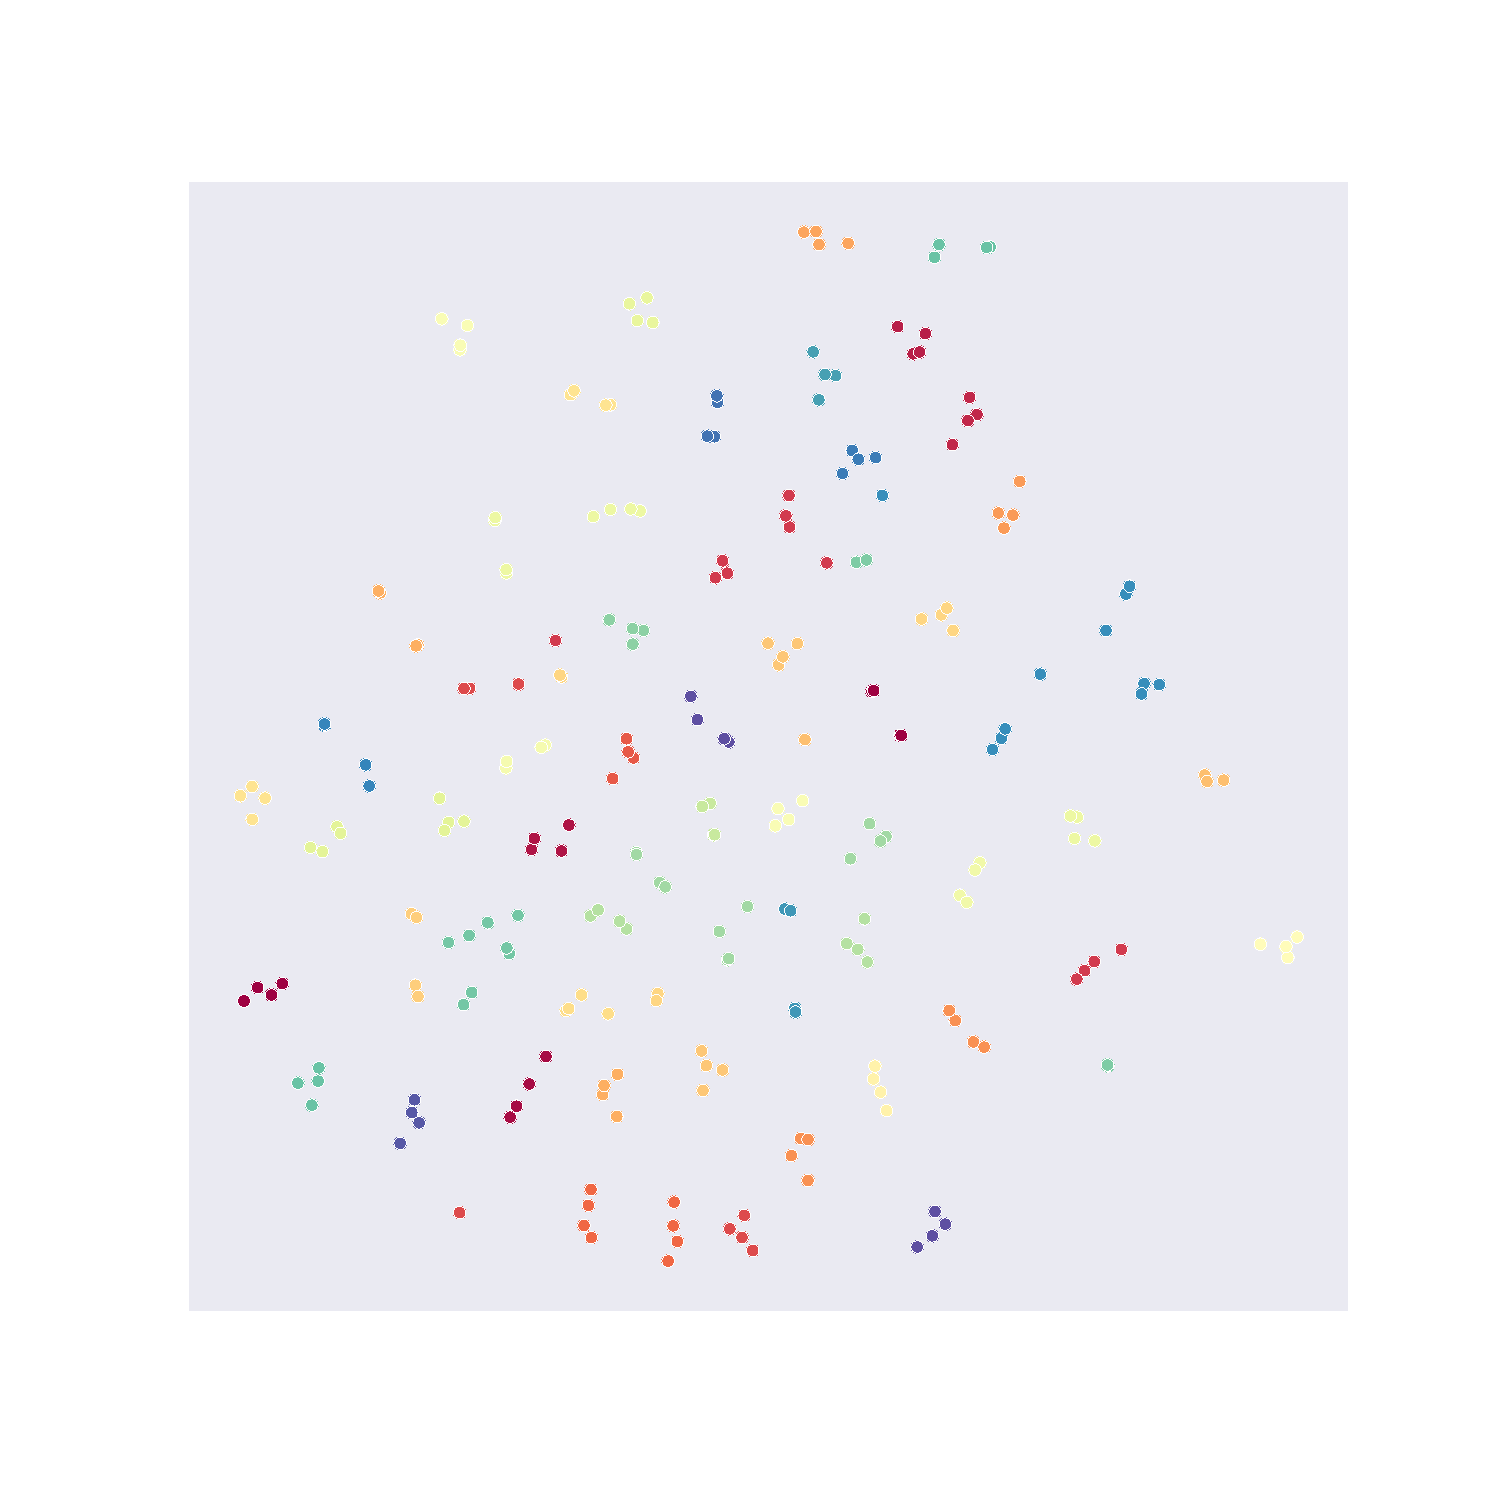
\includegraphics[width=\textwidth,trim=2.55cm 3cm 2.6cm 2.6cm, clip]{chapters/assets/samptr_extra/cnn_emb.pdf}
         \caption{CNN features.}
     \end{subfigure}
     \hspace{1cm}
     \begin{subfigure}[b]{0.4\textwidth}
         \centering
         \captionsetup{justification=centering}
         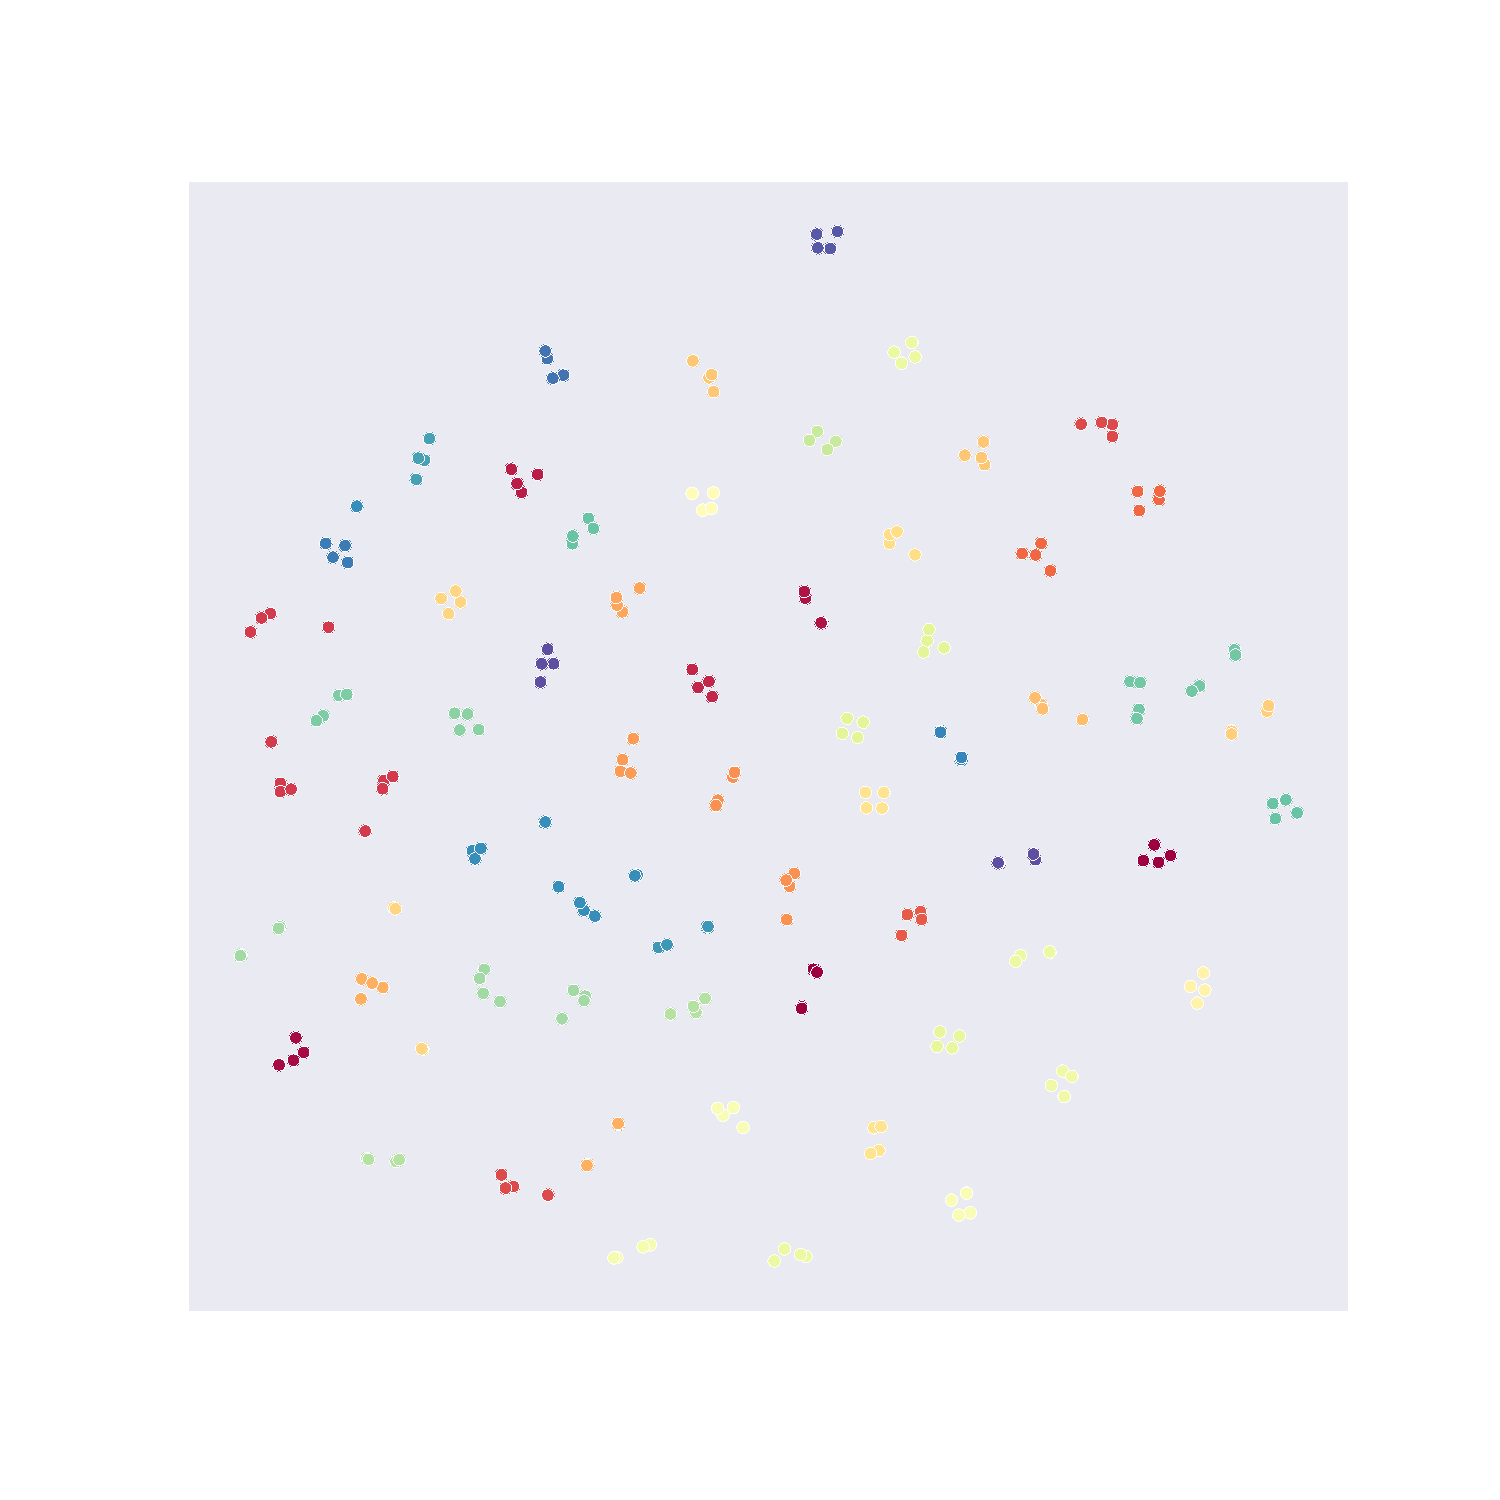
\includegraphics[width=\textwidth, trim=2.55cm 3cm 2.6cm 2.6cm, clip]{chapters/assets/samptr_extra/gnn_emb.pdf}
         \caption{\samp{} refined features.}
     \end{subfigure}
     \caption{ Each point is an image representation that has three neighbours which are its augmentations. The UMAP plot on the left shows features generated by the Conv$4$b backbone, the points are clearly more spread out. The flattened output of the Conv$4$b backbone are used as input to the \samp{} layer. The UMAP plot on the right generated by using the \samp{} layer outputs.
     }
     \label{fig:samp-training-emb-plots}
\end{figure}
\begin{figure}[t]
     \centering
     \begin{subfigure}[b]{0.4\textwidth}
         \centering
         \captionsetup{justification=centering}
         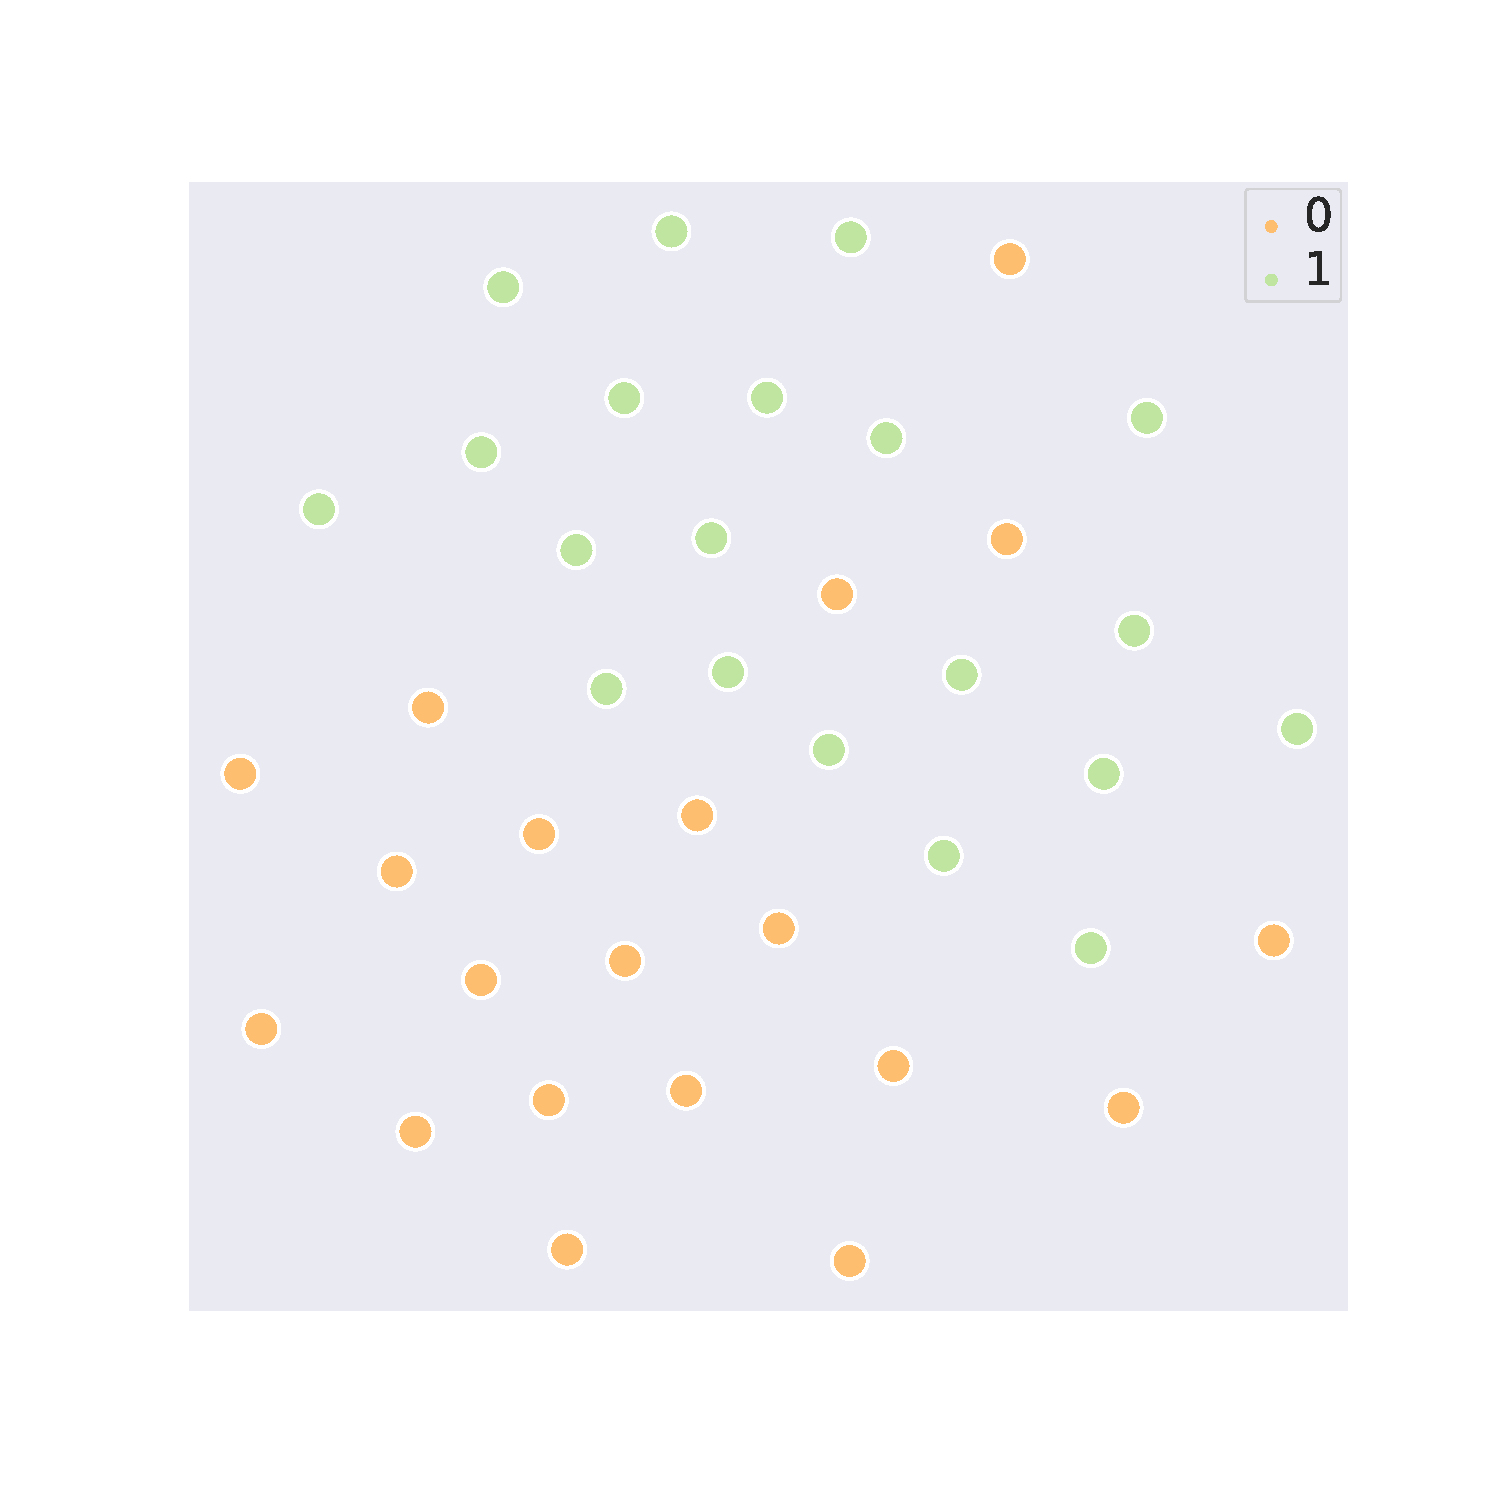
\includegraphics[width=\textwidth,trim=2.55cm 3cm 2.6cm 2.6cm, clip]{chapters/assets/samptr_extra/cnn_val_emb.pdf}
         \caption{UMAP plot of CNN features.}
     \end{subfigure}
     \hspace{1cm}
     \begin{subfigure}[b]{0.4\textwidth}
         \centering
         \captionsetup{justification=centering}
         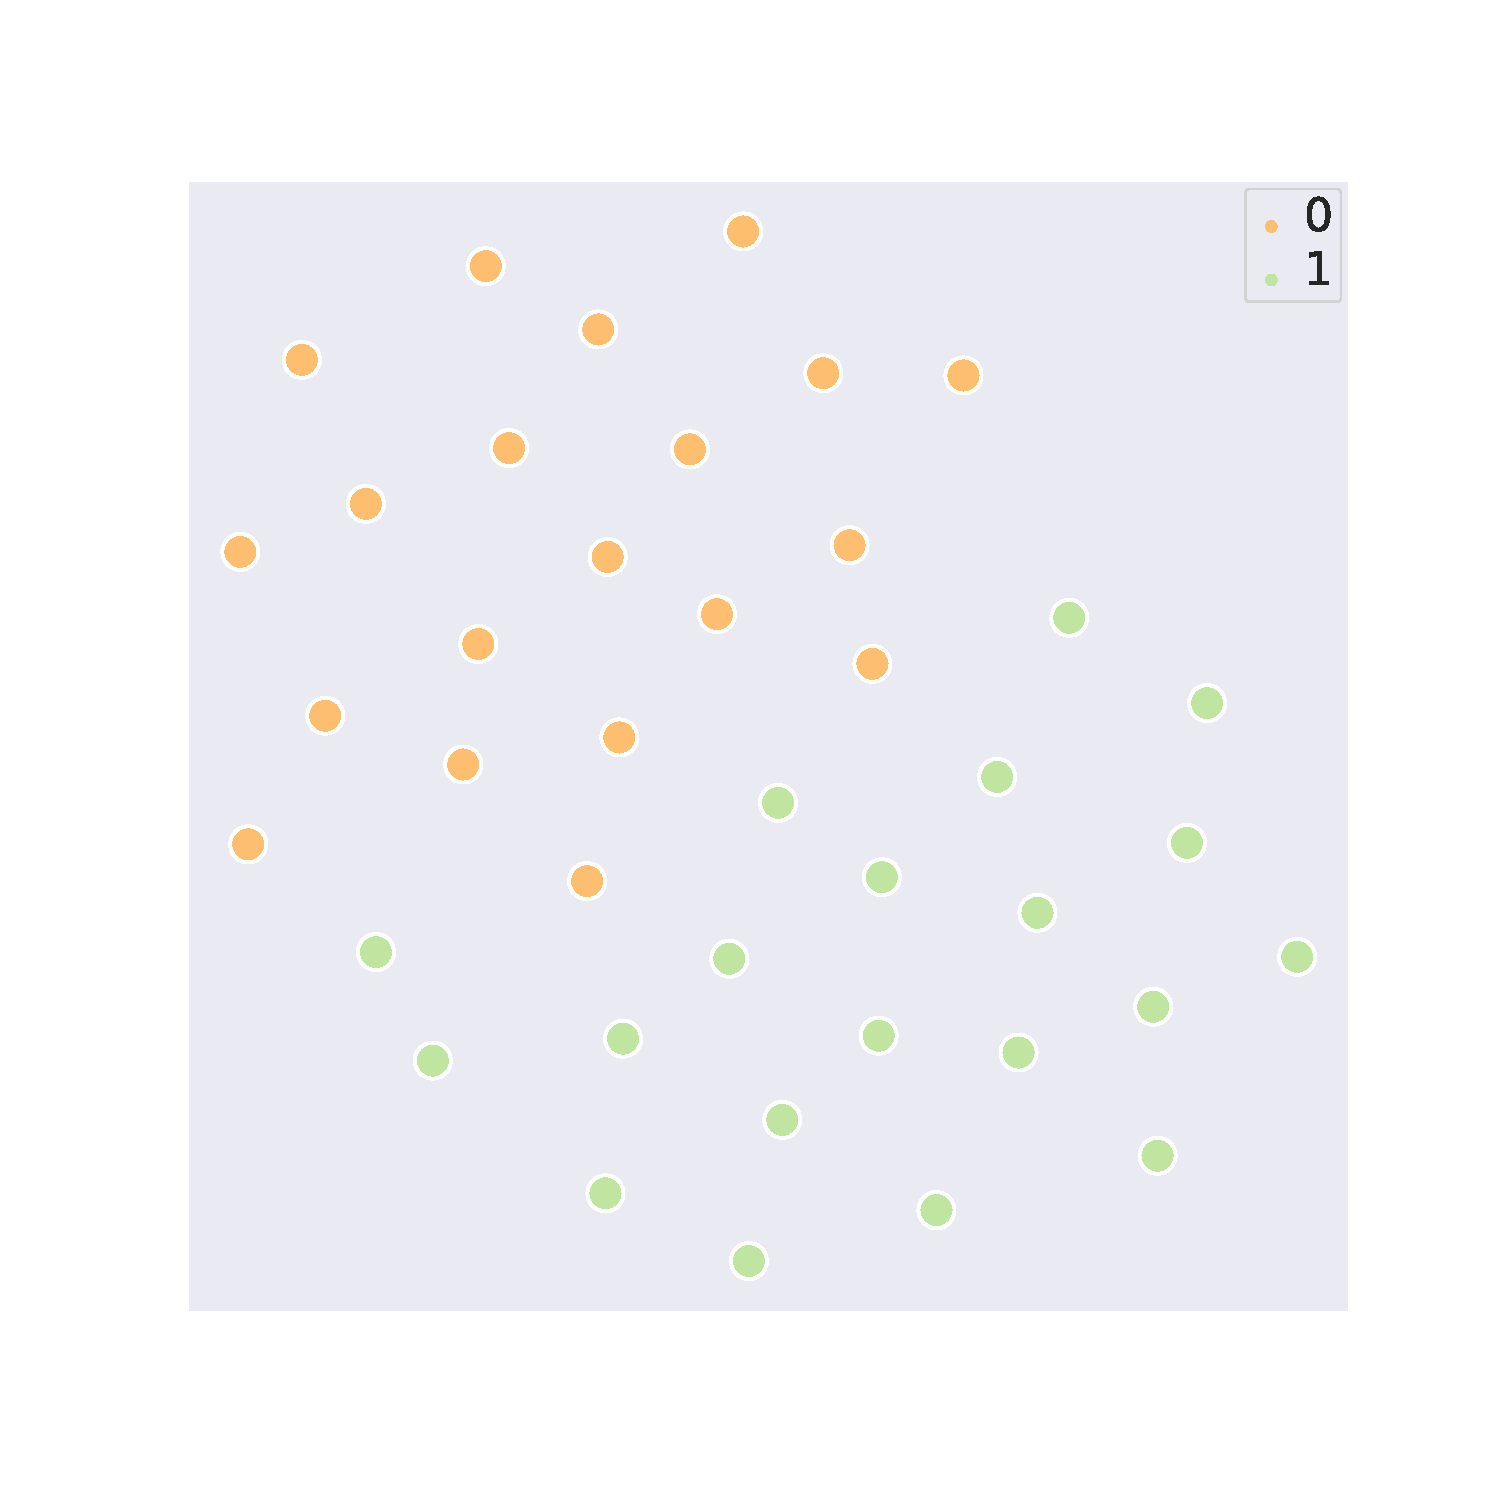
\includegraphics[width=\textwidth, trim=2.55cm 3cm 2.6cm 2.6cm, clip]{chapters/assets/samptr_extra/gnn_val_emb.pdf}
         \caption{UMAP plot of \samp{} refined features.}
     \end{subfigure}
     \caption{The figure on the left shows the CNN features of a support and query set from (\nwks{2}{5}) task drawn from the \miniImagenet{} validation set. Note that there are $15$ query samples per class.
     The figure on the right shows the \samp{} refined features where we can see two clearly separated clusters of points whereas on the right there are a few stray \textcolor{orange}{orange} points. We choose $N=2$ so that the effect of \samp{} is more prominent and immediately visible.}
     \label{fig:samp-val-emb-plots}
\end{figure}
In \cref{fig:samp-training-emb-plots} the plot on the right shows image augmentations tightly grouped around the source image. From this we can infer that the \samp{} layer is capable of recognising similar images and refine their features so that they are closer in the representation space.

Similar to \cref{fig:samp-training-emb-plots}, \cref{fig:samp-val-emb-plots} shows the embeddings of a support and query set in a (\nwks{2}{5}) task. We can see that the CNN features on the left are not as separable, several \textcolor{orange}{orange} dots are in the area of the \textcolor{green}{green} cluster. However, when the CNN features are passed through a \samp{} layer, we can see that the resulting clusters are almost perfectly separable, indicating that the \samp{} layer is working by looking beyond single instances and has learnt to refine features as required. The legend is not shown as there $64$ classes on the figure.

\section{Shortcomings of \samptr{}}\label{sec:samptr-shortcomings}
Although \samptr{} puts forth an impressive performance, there are still some problems that need to be addressed.

\subsection{Reliance on Batch Size}\label{ssec:reliance-on-bsize}
Like other contrastive learning approaches, such as SimCLR \parencite{chen2020simple}, \samptr{} too needs a reasonable batch size to be performant. 
SimCLR achieves its best performance with a batch size of $8192$ \parencite{chen2020simple}, similarly we too notice that as our batch size is increased from $64$ to $128$ there is a noticeable benefit. This is because a larger batch size means access to a greater number of negative pairs that can be used in the contrastive loss. Some methods like MoCo \parencite{he2020momentum} and NNCLR \parencite{dwibedi2021little} make use of a memory module that helps reduce the dependence on batch size.

\subsection{Loss of Spatial Information}\label{ssec:loses-spatial-info}
Currently, the \samp{} layers work on the flattened feature maps generated by the convolutional encoder. Although, this design is not inherently wrong it does lose the spatial information present in the $2$-d feature maps. For example, this could be important when working on features extracted from two images depicting a cat and a bobcat\footnote{\url{https://www.nationalgeographic.com/animals/mammals/facts/bobcat}}. Information regarding the specifics about the shape of their ears or body could all be lost with the flattening operation.

\begin{table}[ht]
        \footnotesize
        \centering
        %over $600$ ($5$-way, $5$-shot) \textit{mini}ImageNet test tasks.}
        % \begin{adjustbox}{width=\columnwidth}
        {\tabcolsep=20pt\def\arraystretch{1}
        \begin{tabularx}{\columnwidth}{l *6{@{\hspace{-5pt}}>{\centering\arraybackslash}X}}
        \toprule
            \textbf{Backbone}& $p$ & $H$ & $L$  & $\beta$ & \textbf{OT} & \textbf{Accuracy} \\
            \midrule
            Conv4b    & 1 & 4 & 64 &  1.0 & \cmark  &  71.42 \scriptsize{$\pm$ 0.73} \\
            Conv4b    & 1 & 4 & 64 &  0.7 & \cmark  &  71.41 \scriptsize{$\pm$ 0.71} \\

            
            Conv4     & 1 & 4 & 64 &  0.7 & \cmark  &  69.61 \scriptsize{$\pm$ 0.71} \\
            Conv4     & 1 & 4 & 64 &  1.0 & \cmark  &  67.60 \scriptsize{$\pm$ 0.62} \\ 
            Conv4     & 1 & 8 & 64 &  1.0 & \cmark  &  63.59 \scriptsize{$\pm$ 0.68} \\ 
            
            Conv4b    & 1 & 4 & 128 & 0.7 & \cmark  &  72.52 \scriptsize{$\pm$ 0.72} \\ 
            Conv4     & 1 & 4 & 128  & 0.7 & \cmark  &  68.33 \scriptsize{$\pm$ 0.71} \\ 
            Conv4     & 1 & 4 & 128 &  0.0  & \cmark  &  52.81 \scriptsize{$\pm$ 0.66} \\
            Conv4b    &	1 &	4 &	128 & 0.0 & \cmark  &  72.44 \scriptsize{$\pm$ 0.69} \\
            \cdashlinelr{1-7}
            Resnet-12 & 1 & 2 & 128 & 0.7  & \cmark & 69.83 \scriptsize{$\pm$ 0.71}\\
            ResNet-18 &	1 & 2 & 128	& 0.7  & \cmark	& 70.91 \scriptsize{$\pm$ 0.69}\\
            ResNet-50 &	1 & 2 & 128 & 0.7 & \cmark  & 74.05 \scriptsize{$\pm$ 0.64}\\
            
            Resnet-12 & 1 & 4 & 128 & 0.7  & \cmark & 71.93 \scriptsize{$\pm$ 0.73}\\
            ResNet-18 &	1 & 4 & 128	& 0.7  & \cmark	& 71.2 \scriptsize{$\pm$ 0.68}\\
            ResNet-50 &	1 & 4 & 128 & 0.7 & \cmark  & 73.27 \scriptsize{$\pm$ 0.68}\\
        \bottomrule
        \end{tabularx}}
        \caption{Ablation study of various parameters on accuracy.}
        \label{tab:samptr-ablation}
\end{table}


\subsection{Poor Scaling with Larger Backbones}\label{ssec:poor-scaling}
We see that \samptr{} scales poorly with larger backbones such as ResNet-$12$, ResNet-$18$, and ResNet-$50$ \parencite{He2015}. The results for these backbones are shown in \cref{tab:samptr-ablation}, which is a slightly modified table present in \cref{chap:samp-transfer-art}. From \cref{tab:samptr-ablation}, we can see that only the largest ResNet, ResNet-$50$ manages to outperform a much smaller Conv$4$b network. 

Although it is natural to presume that scaling to a larger backbone would also improve performance \parencite{He2015,Goyal2021}, we see the opposite in action here. We hypothesise that this could be due to sub-optimal hyperparameters, including the choice of optimiser. However, due to the lack of time and resources, we were unable to extensively investigate this behaviour.